\chapter{Scaling up the models}
\label{chap:deep_cnns}

\begin{supportbox}{About this chapter}
We now turn to the task of designing differentiable models having dozens (or hundreds) of layers. As we saw, the receptive field of convolutional models grows linearly with the number of layers, motivating architectures with such depth. This can be done by properly stabilizing training using a plethora of methods, ranging from data augmentation to normalization of the hidden states.
\end{supportbox}


\section{The ImageNet challenge}

Let us consider again the task of image classification, which holds a strong interest for neural networks, both practically and historically. In fact, interest in these models in the period 2012-2018 can be associated in large part to the \textbf{ImageNet Large Scale Visual Recognition Challenge}\footnote{\url{https://image-net.org/challenges/LSVRC/}} (later \textbf{ImageNet} for simplicity). ImageNet was a yearly challenge that run from 2010 to 2017 to evaluate state-of-the-art models for image classification. The challenge was run on a subset of the entire ImageNet dataset, consisting of approximately 1M images tagged across 1k classes. 

It is instructive to take a look at the early editions of the challenges. In 2010\footnote{\url{https://image-net.org/challenges/LSVRC/2010/}} and in 2011,\footnote{\url{https://image-net.org/challenges/LSVRC/2011/}} the winners were linear kernels methods built with a combination of specialized image descriptors and kernels, with a top-5\% error of 28\% (2010) and 26\% (2011). Despite a number of promising results,\footnote{\url{https://people.idsia.ch/~juergen/computer-vision-contests-won-by-gpu-cnns.html}} convolutional models trained by gradient descent remained a niche topic in computer vision. Then, In 2012 the winner model (AlexNet, \cite{krizhevsky2012imagenet}) achieved a top-5\% error of 15.3\%, 10\% lower than all (non-neural) competitors. 

This was followed by a veritable “Copernican revolution” (apologies to Copernicus) in the field, since in a matter of a few years almost all submissions turned to convolutional models, and the overall accuracy grew at an unprecedented speed, upward of 95\% (leading to the end of the challenge in 2017), as shown in Figure \ref{fig:papers_with_code}. In a span of 5 years, convolutional models trained with gradient descent became the leading paradigm in computer vision, including other subfields we are not mentioning here, from object detection to semantic segmentation and depth estimation.

\begin{SCfigure}
    \centering
    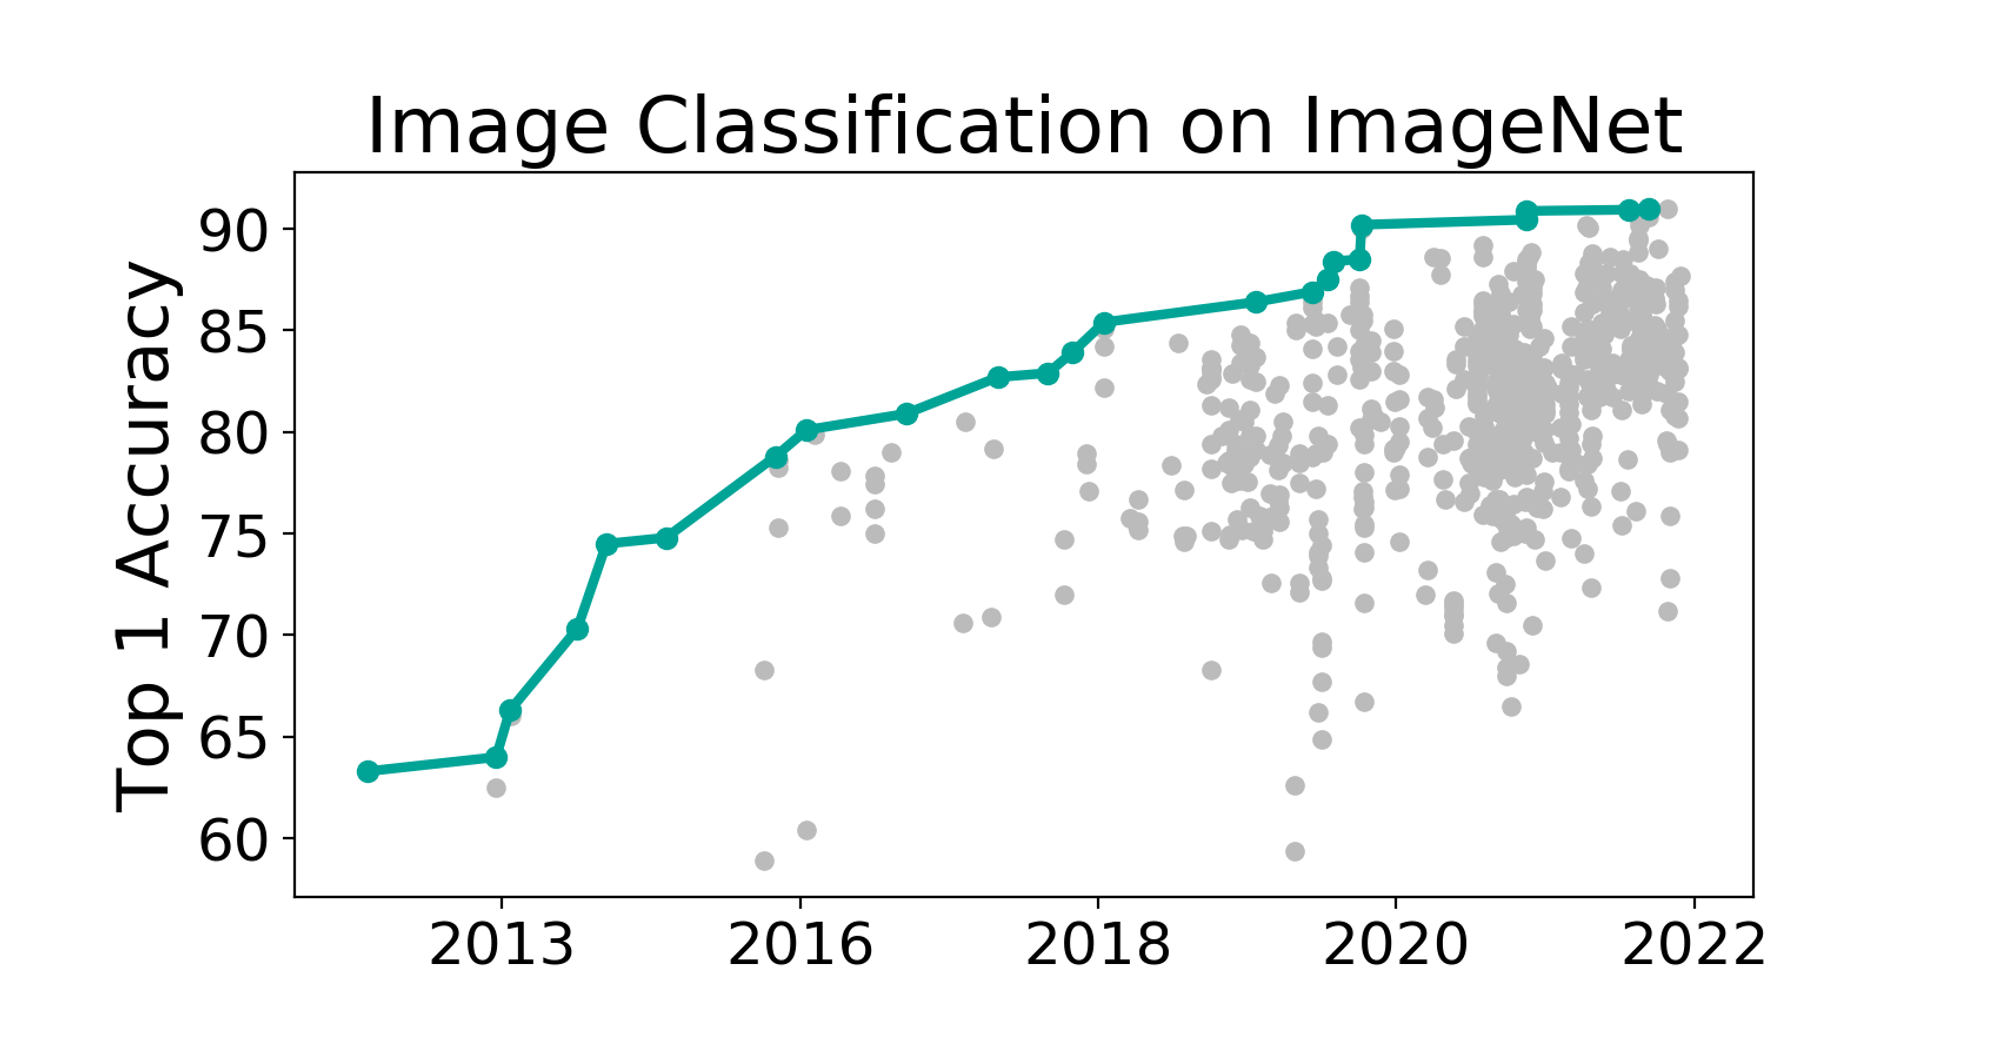
\includegraphics[width=0.6\textwidth]{images/imagenet}
    \caption[Reproduced from Papers With Code.]{Top-$1$ accuracy on the ImageNet dataset. Reproduced from Papers With Code.\footnote{\url{https://paperswithcode.com/}}}
    \label{fig:papers_with_code}
\end{SCfigure}

AlexNet was a relatively simple model consisting of 5 convolutional layers and 3 fully-connected layers, totaling approximately 60M parameters, while the top-performing models in Figure \ref{fig:papers_with_code} require up to hundreds of layers. This is basic example of a scaling law (Chapter \ref{chap:introduction}): adding layers and compute power for training is proportionally linked to the accuracy of the model up to a saturation point given by the dataset. However, scaling up convolutional models beyond a few layers is non-trivial, as it runs into a number of problems ranging from slow optimization to gradient issues and numerical instabilities. As a consequence, a large array of techniques were developed in 2012-2017 to stabilize training of very large models.

In this chapter we provide an overview of some of these techniques. We focus on ideas and methods that are still fundamental nowadays, even for other architectures (e.g., transformers). We begin by three techniques to improve training that are well-known in machine learning: \textbf{weight regularization}, \textbf{data augmentation}, and \textbf{early stopping}. Then, we describe three of the most influential techniques popularized in 2012-2017: \textbf{dropout}, \textbf{batch normalization}, and \textbf{residual connections}, more or less in chronological order of introduction. For each method we describe the basic algorithm along with some variants that work well in practice (e.g., layer normalization).


\section{Data and training strategies}

\subsection{Weight regularization}

One possible way to improve training is to penalize solutions that may seem unplausible, such as having one or two extremely large weights. Denote by $\mathbf{w}$ the vector of all parameters of our model, and by $L(\mathbf{w}, \mathcal{S}_n)$ the loss function on our dataset (e.g., average cross-entropy). We can formalize the previous idea by defining a so-called \textbf{regularization term} $R(\mathbf{w})$ that scores solutions based on our preference, and penalize the loss by adding the regularization term to the original loss function:
%
$$
L_{\text{reg}}=L(\mathbf{w}, \mathcal{S}_n)+\lambda R(\mathbf{w})
$$
%
where we assume that a higher value of $R(\mathbf{w})$ corresponds to a worse solution, and $\lambda \ge 0$ is a scalar that weights the two terms. For $\lambda=0$ the regularization term has no effect, while for $\lambda \rightarrow \infty$ we simply select the best function based on our a priori knowledge.

This can also be justified as performing maximum a-priori (instead of maximum likelihood) inference based on the combination of a prior distribution on the weights $p(\mathbf{w})$ and a standard likelihood function on our data (Section \ref{sec:bayesian_learning}):
%
\begin{equation}
\mathbf{w}^*=\underset{\mathbf{w}}{\arg\max}\left\{ \log p(\mathcal{S}_n \;\vert\; \mathbf{w}) + \log p(\mathbf{w})\right\}
\label{eq:map_solution}
\end{equation}
%
where having a regularization term corresponds to a non-uniform prior distribution $p(\mathbf{w})$. We have already seen one example of regularization in Section \ref{subsec:regularizing_least_squares}, i.e., the $\ell_2$ norm of the weights:
%
$$
R(\mathbf{w})=\lVert \mathbf{w} \rVert^2 =\sum_i w_i^2
$$
%
For the same unregularized loss, penalizing the $\ell_2$ norm will favor solutions with a lower weight magnitude, corresponding to “less abrupt” changes in the output for a small deviation in the input.\footnote{With respect to \eqref{eq:map_solution},  $\ell_2$ regularization is equivalent to choosing a Gaussian prior on the weights with diagonal $\sigma^2 \mathbf{I}$ covariance.} Consider now the effect of the regularization term on the gradient term:
%
$$
\nabla L_{\text{reg}}=\nabla L(\mathbf{w},\mathcal{S}_n)+2\lambda\mathbf{w}
$$
%
Written in this form, this is sometimes called \textbf{weight decay}, because absent the first term, its net effect is to decay the weights by a small proportional factor $\lambda$ (sending them to $0$ exponentially fast in the number of iterations if $\nabla L(\mathbf{w}, \mathcal{S}_n)=0$). For (S)GD, $\ell_2$ regularization and weight decay coincide. However, for other types of optimization algorithms (e.g., momentum-based SGD, Adam), a post-processing is generally applied on the gradients. Denoting by $g(\nabla L(\mathbf{w}, \mathcal{S}_n))$ the post-processed gradients of the (unregularized) loss, we can write a generalized weight decay formulation (ignoring the constant term $2$) as:

$$
\mathbf{w}_t =\mathbf{w}_{t-1} \eqnmarkbox[drawred]{node}{-g(\nabla L(\mathbf{w}_{t-1}, \mathcal{S}_n))} \eqnmarkbox[drawgreen]{node2}{- \lambda \mathbf{w}_{t-1}}
$$
\annotate[yshift=1em]{above,right}{node}{Unregularized gradient}
\annotate[yshift=-1em]{below,right}{node2}{Weight decay term}

This is different from pure $\ell_2$ regularization, in which case the gradients of the regularization term would be inside $g(\cdot)$. This is especially important for algorithms like Adam, for which the weight decay formulation can work better \cite{loshchilov2018fixing}.

We can also consider other types of regularization terms. For example, the $\ell_1$ norm:
%
$$
R(\mathbf{w})=\lVert \mathbf{w} \rVert_1=\sum_i \lvert x_i \rvert
$$
%
can favor \textit{sparse} solutions having a high percentage of zero values (and it corresponds to placing a Laplace prior on the weights). This can also be generalized to group sparse variants to enforce structured sparsity on the neurons \cite{scardapane2017group}.\footnote{Training sparse models is a huge topic with many connections also to efficient hardware execution. See \cite{bach2012optimization} for a review on sparse penalties in the context of convex models, and \cite{hoefler2021sparsity} for an overview of sparsity and pruning in general differentiable models.}  Sparse $\ell_1$ penalization is less common than for other machine learning models because it does not interact well with the strong non-convexity of the optimization problem and the use of gradient descent \cite{ziyin2023spred}. However, it is possible to re-parameterize the optimization problem to mitigate this issue at the cost of a larger memory footprint. In particular, \cite{ziyin2023spred}  showed that we can replace $\mathbf{w}$ with two equivalently shaped vectors $\mathbf{a}$ and $\mathbf{b}$, and:
%
\begin{equation}
\mathbf{w} = \mathbf{a} \odot \mathbf{b} \;,\; \lVert \mathbf{w} \rVert_1 \approx \lVert \mathbf{a} \rVert^2 + \lVert \mathbf{b} \rVert^2
\end{equation}
%
where $\approx$ means that the two problems can be shown to be almost equivalent under very general conditions \cite{ziyin2023spred}.

We can gain some geometric insights as to why (and how) regularization works by considering a convex loss function $L(\cdot, \cdot)$ (e.g., least-squares), in which case the regularized problem can be rewritten in an explicitly constrained form as:
%
\begin{equation}
\begin{matrix}\arg\min & L(\mathbf{w}, \mathcal{S}_n) \\ \text{subject to} & R(\mathbf{w})\le\mu \end{matrix}
\label{eq:constrained_problem}
\end{equation}

where $\mu$ depends proportionally on $\lambda$, with the unconstrained formulation arising by rewriting \eqref{eq:constrained_problem} with a Lagrange multiplier. In this case, $\ell_2$ regularization corresponds to constraining the solution to lie inside a circle centered in the origin, while $\ell_1$ regularization corresponds to having a solution inside (or on the vertices) of a regular polyhedron centered in the origin, with the sparse solutions lying at the vertices intersecting the axes.

\subsection{Early stopping}

From the point of view of optimization, minimizing a function $L(\mathbf{w})$ is the task of finding a stationary point as quickly as possible, i.e., a point $\mathbf{w}_t$ such that $\nabla L(\mathbf{w}_t) \approx 0$:

$$
\lVert L(\mathbf{w}_t)-L(\mathbf{w}_{t-1})\rVert^2\le\varepsilon
$$

for some tolerance $\varepsilon > 0$. However, this does not necessarily correspond to what we want when optimizing a model. In particular, in a low-data regime training for too long can incur in overfitting and, in general, anything which improves generalization is good irrespective of its net effect on the value on $L(\cdot)$ or the descent direction (e.g., weight decay).

\textbf{Early stopping} is a simple example of the difference between pure optimization and learning. Suppose we have access to a small supervised dataset, separate from the training and test dataset, that we call \textbf{validation dataset}. At the end of every epoch, we track a metric of interest on the validation dataset, such as the accuracy or the F1-score. We denote the score at the $t$-th epoch as $a_t$. The idea of early stopping is to check this metric to see if it keeps improving: if not, we may be entering an overfitting regime and we should stop training. Because the accuracy can oscillate a bit due to random fluctuations, we do this robustly by considering a window of $k$ epochs (the \textbf{patience}):

$$
\text{If } a_t \le a_i ,\;\; \eqnmarkbox[drawred]{node}{\forall i =t-1,t-1, \ldots,t-k} \rightarrow \text{Stop training}
$$
\annotate[yshift=-1em]{below,left}{node}{Wait for $k$ epochs}

\vspace{1em}
For a high value of the patience hyper-parameter $k$, the algorithm will wait more, but we will be more robust to possible oscillations. If we have a mechanism to store the weights of the model (\textbf{checkpointing}) we can also rollback the weights to the last epoch that showed improvement, corresponding to the epoch number $t-k$.

Early stopping can be seen as a simple form of \textbf{model selection}, where we select the optimal number of epochs based on a given metric. Differently from the optimization of the model, we can optimize here for any metric of interest, such as the F1-score, even if not differentiable. 

Interestingly, for large over-parameterized models early stopping is not always beneficial, as the relation between epochs and validation error can be non-monotone with multiple phases of ascent and descent (a phenomenon called \textbf{multiple descents} \cite{rocks2022memorizing}) and sudden drops in the loss after long periods of stasis \cite{power2022grokking}. Hence, early stopping is useful mostly when optimizing on small datasets.

\subsection{Data augmentation} \addclock

Generally speaking, the most effective method to improve performance for a model is to increase the amount of available data. However, labelling data can be costly and time-consuming, and generating data artificially (e.g., with the help of large language models) requires customized pipelines to work effectively \cite{patel2024datadreamer}.

In many cases, it is possible to partially mitigate this issue by \textit{virtually} increasing the amount of available data by transforming them according to some pre-specified number of (semantic preserving) transformations. As a simple example, consider a vector input $\mathbf{x}$ and a transformation induced by adding Gaussian noise:
%
$$
\mathbf{x}^\prime=\mathbf{x}+\varepsilon,\;\varepsilon \sim \mathcal{N}(\mathbf{0},\sigma^2\mathbf{I})
$$
%
This creates a virtually infinite amount of data comprised in a small ball centered around $\mathbf{x}$. In addition, this data must not be stored in the disk, and the process can be simulated by applying the transformation at runtime every time a new mini-batch is selected. In fact, it is known that training in this way can make the model more robust and it is connected to $\ell_2$ regularization \cite{bishop1995training}. However, vectorial data is unstructured, and adding noise with too high variance can generate points that are invalid.

For images, we can do better by noting that there is in general a large number of transformations that can change an image while preserving its semantic: zooms, rotations, brightness modifications, contrast changes, etc. Denote by $T(x; c)$ one such transformation (e.g., rotation), parameterized by some parameter $c$ (e.g., the rotation angle). Most transformations include the base image as a special case (in this case, for example, with a rotation angle $c=0$). \textbf{Data augmentation} is the process of transforming images during training according to one or more of these transformations:
%
\begin{equation}
x^\prime=T(x;c),\;c\sim p(c)
\label{eq:data_augmentation}
\end{equation}
%
where $p(c)$ denotes the distribution of all valid parameters (e.g., rotation angles between $-20^\circ$ and $+20^\circ$). During training, each element of the dataset is sampled once per epoch, and each time a different transformation \eqref{eq:data_augmentation} can be applied, creating a (virtually) unlimited stream of unique data points.

Data augmentation is very common for images (or similar data, such as audio and video), but it requires a number of design choices: what transformations to include, which parameters to consider, and how to compose these transformations. A simple strategy called \textbf{RandAugment} \cite{cubuk2020randaugment} considers a wide set of transformations, and for every mini-batch samples a small number of them (e.g., 2 or 3), to be applied sequentially with the same magnitude. Still, the user must verify that the transformations are valid (e.g., if recognizing text, horizontal flipping can make the resulting image invalid). From a practical point of view, data augmentation can be included either as part of the data loading components (see Box \ref{code:data_augmentation}), or as part of the model.

\begin{mypy}{Data augmentation pipeline with two transformations applied in sequence, taken from the {\footnotesize\mintinline{python}{torchvision}} package. In PyTorch, augmentations can be passed to the data loaders or used independently. In other frameworks, such as TensorFlow and Keras, data augmentation can also be included natively as layers inside the model.}{code:data_augmentation}
# Image tensor (batch, channels, height, width)
img = torch.randint(0, 256, size=(32, 3, 256, 256))

# Data augmentation pipeline
from torchvision.transforms import v2
transforms = v2.Compose([
    v2.RandomHorizontalFlip(p=0.5),
    v2.RandomRotation(10),
])

# Applying the data augmentation pipeline: each function 
# call returns a different mini-batch starting from the 
# same input tensor.
img = transforms(img)
\end{mypy}

Data augmentation pipelines and methods can be more complex than simple intuitive transformations. Even for more sophisticated types, the intuition remains that, as long as the model is able to solve a task in a complex scenario (e.g., recognizing an object in all brightness conditions) it should perform even better in a realistic, mild scenario. Additionally, data augmentation can prevent overfitting by avoiding the repetition of the same input multiple times.

As an example of more sophisticated methods, we describe \textbf{mixup} \cite{zhang2017mixup} for vectors, and its extension \textbf{cutmix} \cite{yun2019cutmix} for images. For the former, suppose we sample two examples, $(\mathbf{x}_1, y_1)$ and $(\mathbf{x}_2, y_2)$. The idea of mixup is to create a new, virtual example which is given by their convex combination:
%
\begin{gather}
\mathbf{x}=\lambda\mathbf{x}_1+(1-\lambda)\mathbf{x}_2\\y=\lambda y_1+(1-\lambda)y_2
\label{eq:mixup}
\end{gather}
%
where $\lambda$ is chosen randomly in the interval $[0,1]$. This procedure should push the model to have a simple (linear) output in-between the two examples, avoiding abrupt changes in output. From a geometric viewpoint, for two points that are close, we can think of \eqref{eq:mixup} as slowly moving on the manifold of the data, by following the line that connects two points as $\lambda$ goes from $0$ to $1$.

Mixup may not work for images, because linearly interpolating two images pixel-by-pixel gives rise to blurred images. With \textbf{cutmix}, we sample instead a small patch of fixed shape (e.g., $32 \times 32$) on the first image. Denote by $\mathbf{M}$ a binary mask of the same shape as the images, with $1$ for pixels inside the patch, and $0$ for pixels outside the patch. In cutmix, we combine two images $x_1$ and $x_2$ by “stitching” a piece from the first one on top of the second one:
%
$$
x=\mathbf{M}\odot x_1+(1-\mathbf{M})\odot x_2
$$
%
while the labels are still linearly interpolated as before with a random coefficient $\lambda$. See Figure \ref{fig:cutmix} for an example of data augmentation using both rotation and cutmix.

\begin{figure}[t]
    \centering
    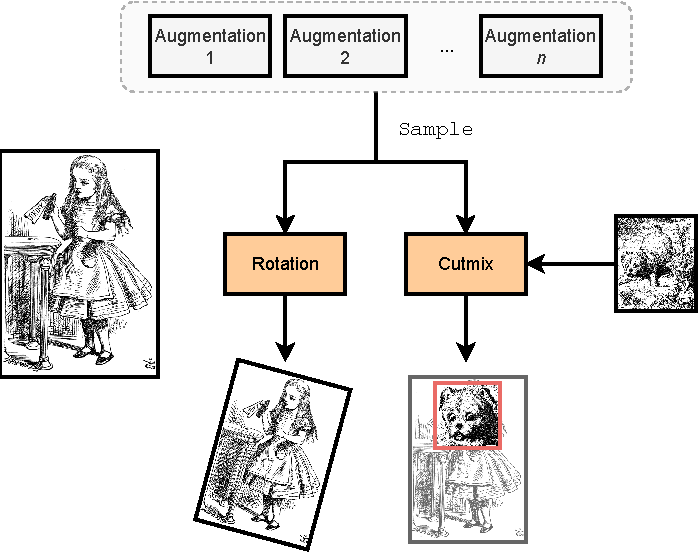
\includegraphics[width=0.7\textwidth]{images/data_augmentation}
    \caption{High-level overview of data augmentation. For every mini-batch, a set of data augmentations are randomly sampled from a base set, and they are applied to the images of the mini-batch. Here, we show an example of \textit{rotation} and an example of \textit{cutmix}. Illustrations by John Tenniel, reproduced from Wikimedia.}
    \label{fig:cutmix}
\end{figure}

\section{Dropout and normalization}

The strategies we have described in the previous section are very general, in the sense that they imply modifications to the optimization algorithm or to the dataset itself, and they can be applied to a wide range of algorithms. 

Instead, we now focus on three ideas that were popularized in the period between 2012 and 2016, mostly in the context of the ImageNet challenge. All three are specific to differentiable models, since they can be implemented as additional layers or connections in the model that simplify training of very deep models. We list the methods in roughly chronological order. As we will see in the remaining sections, these methods remain fundamental also beyond convolutional models.

\subsection{Regularization via dropout}
\label{subsec:dropout}

When discussing data augmentation, we mentioned that one insight is that augmentation forces the network to learn in a more difficult setup, so that its performance in a simpler environment can improve in terms of accuracy and robustness. \textbf{Dropout} \cite{srivastava2014dropout} extends this idea to the internal embeddings of the model: by artificially introducing noise during training to the intermediate outputs of the model, the solution can improve.

There are many choices of possible noise types: for example, training with small amounts of Gaussian noise in the activation has always been a popular alternative in the literature of recurrent models. As the name suggests, dropout's idea is to randomly remove certain units (neurons) during the computation, reducing the dependence on any single internal feature and (hopefully) leading to training robust layers with a good amount of redundancy.

\begin{figure}
    \centering
    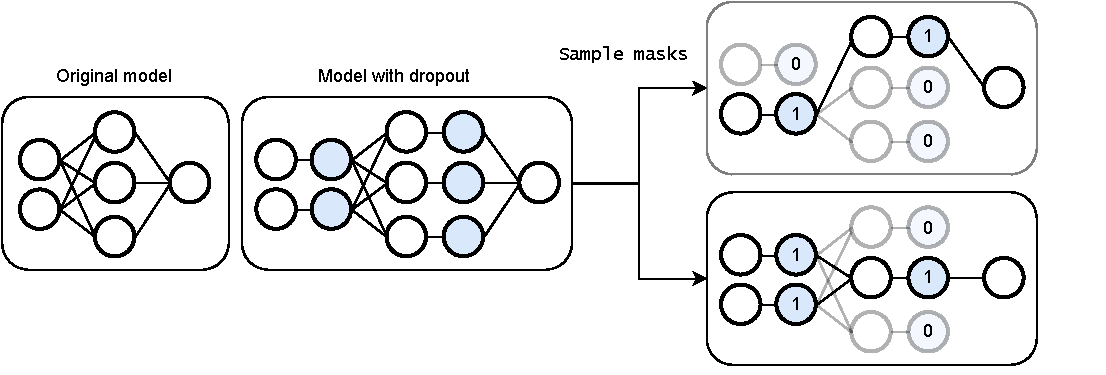
\includegraphics[width=0.95\textwidth]{images/dropout}
    \caption{Schematic overview of dropout: starting from a base model, we add additional units after each layer of interest, shown in blue. At training time, each dropout unit is randomly assigned a binary value, masking part of the preceding layers. Hence, we select one out of exponentially many possible models having a subset of active hidden units every time a forward pass is made. Dropout can also be applied at the input level, by randomly removing some input features.}
    \label{fig:dropout}
\end{figure}

We define dropout in the case of a fully-connected layer, which is its most common use case. 

\begin{definition}[Dropout layer] \addbottle
%
Denote by $\mathbf{X} \sim (n, c)$ a mini-batch of internal activations of the model (e.g., the output of some intermediate fully-connected layer) with $n$ elements in the mini-batch and $c$ features. In a dropout layer, we first sample a binary matrix $\mathbf{M} \sim \text{Binary}(n,c)$ of the same size, whose elements are drawn from a Bernoulli distribution with probability $p$ (where $p \in [0,1]$ is a user’s hyper-parameter):\footnote{The samples from $\text{Bern}(p)$ are $1$ with probability $p$ and $0$ with probability $1-p$.}
%
\begin{equation}
M_{ij}\sim \text{Bern}(p)
\label{eq:sampling_m}
\end{equation}
%
The output of the layer is obtained by masking the input:
%
$$
\textnormal{Dropout}(\mathbf{X})=\mathbf{M} \odot \mathbf{X}
$$
%
The layer has a single hyper-parameter, $p$, and no trainable parameters.
%
\end{definition}
%
We call $1-p$ the \textbf{drop probability}. Hence, for any element in the mini-batch, a random number of units (approximately $(1-p) \%$) will be set to zero, effectively removing them. This is shown in Figure \ref{fig:dropout}, where the additional dropout units are shown in blue. Sampling the mask is part of the layer’s forward pass: for two different forward passes, the output will be different since different elements will be masked, as shown on the right in Figure \ref{fig:dropout}. 

As the figure shows, we can implement dropout as a layer, which is inserted after each layer that we want to drop. For example, consider the fully-connected model with two layers shown in Figure \ref{fig:dropout}:
%
$$
y=(\text{FC}\circ\text{FC})(\mathbf{x})
$$
%
Adding dropout regularization over the input and over the output of the first layer returns a new model having \textit{four} layers:
%
$$
y=(\text{FC}\circ{\color{drawred}\text{Dropout}}\circ\text{FC} \circ {\color{drawred}\text{Dropout}})(\mathbf{x})
$$
%
See Box \ref{code:dropout_model} for an implementation in PyTorch.

\begin{mypy}{The model in Figure \ref{fig:dropout} implemented as a sequence of four layers in PyTorch. During training, the output of the model will be stochastic due to the presence of the two dropout layers.}{code:dropout_model}
model = nn.Sequential(
    nn.Dropout(0.3),
    nn.Linear(2, 3), nn.ReLU(),
    nn.Dropout(0.3),
    nn.Linear(3, 1)
)
\end{mypy}

While dropout can improve the performance, the output $y$ is now a random variable with respect to the sampling of the different masks inside the dropout layers, which is undesirable after training. For example, two forward passes of the network can return two different outputs, and some draws (e.g., with a very large number of zeroes) can be suboptimal. Hence, we require some strategy to replace the forward pass with a deterministic operation. 

Suppose we have $m$ dropout layers. Let us denote by $\mathbf{M}_i$ the mask in the $i$-th dropout layer, by $p(\mathbf{M}_1, \ldots, \mathbf{M}_m) = \prod_{i=1}^m p(\mathbf{M}_i)$ the probability distribution over the union of the masks, and by $f(\mathbf{x}; \mathbf{M})$ the deterministic output once a given set of masks $\mathbf{M} \sim p(\mathbf{M})$ are chosen. One choice is to replace the dropout effect with its expected value during inference:
%
$$
f(\mathbf{x})=\begin{cases} f(\mathbf{x}; \mathbf{M}), \;\; \mathbf{M}\sim p(\mathbf{M}) & \texttt{ [training]} \\ \mathbb{E}_{p(\mathbf{M})}\left[f(\mathbf{x}; \mathbf{M})\right]  & \texttt{ [inference]}\end{cases}
$$
%
We can approximate the expected value via Monte Carlo sampling (Appendix \ref{chap:probability_theory}) by repeatedly sampling masks values and averaging:
%
$$
\mathbf{E}_{p(\mathbf{M})}\left[f(\mathbf{x}; \mathbf{M})\right] \approx \frac{1}{k}\sum_{i=1}^k f(\mathbf{x}; \mathbf{Z}_i),\;\; \mathbf{Z}_i \sim p(\mathbf{M})
$$
%
which is simply the average of $k$ forward passes. This is called \textbf{Monte Carlo dropout} \cite{gal2016dropout}. The output is still stochastic, but with a proper choice of $k$, the variance can be contained. In addition, the outputs of the different forward passes can provide a measure of uncertainty over the prediction. 

However, performing multiple forward passes can be expensive. A simpler (and more common) option is to replace the random variables \textit{layer-by-layer}, which is a reasonable approximation. The expected value in this case can be written in closed form:
%
$$
\mathbb{E}_{p(\mathbf{M})}\left[\text{Dropout}(\mathbf{X})\right]=p\mathbf{X}
$$
%
which is the input rescaled by a constant factor $p$ (the probability of sampling a $1$ in the mask). This leads to an even simpler formulation, \textbf{inverted dropout}, where this correction is accounted for during training:
%
$$
\text{Dropout}(\mathbf{X})=\begin{cases} \displaystyle\frac{\mathbf{M}\odot\mathbf{X}}{(1-p)} & \texttt{ [training]} \\ \,\,\mathbf{X}  & \texttt{ [inference]}\end{cases}
$$
%
In this case, the dropout layer has no effect when applied during inference and can be directly removed. This is the preferred implementation in most frameworks. See Box \ref{code:dropout} for some comparisons.

\begin{mypy}{Applying the model from Box \ref{code:dropout_model} on a mini-batch of $16$ examples. For layers like dropout, a framework requires a way to differentiate between a  forward pass executed during training or during inference. In PyTorch, this is done by calling the {\footnotesize\mintinline{python}{train}} and {\footnotesize\mintinline{python}{eval}} methods of a model, which set an internal {\footnotesize\mintinline{python}{train}} flag on all layers. We also show a vectorized implementation of Monte Carlo dropout.}{code:dropout}
x = torch.randn((16, 2))

# Training with dropout
model.train()
y = model(x)

# Inference with dropout
model.eval()
y = model(x)

# Monte Carlo dropout for inference
k = 10
model.train()
y = model(x[:, None, :].repeat(1, k, 1)).mean(1)
\end{mypy}

As we mentioned, dropout (possibly with a low drop probability, such as $p=0.1$ or $p=0.2$) is common for fully-connected layers. It is also common for attention maps (introduced in the next chapter). It is less common for convolutional layers, where dropping single elements of the input tensor results in sparsity patterns which are too unstructured. Variants of dropout have been devised which take into consideration the specific structure of images: for example, \textbf{spatial dropout} \cite{tompson2015efficient} drops entire channels of the tensor, while \textbf{cutout} \cite{devries2017improved} drops spatial patches of a single channel.

Other alternatives are also possible. For example, \textbf{DropConnect} \cite{wan2013regularization} drops single weights of a fully-connected layer:
%
$$
\text{DropConnect}(\mathbf{x})=(\mathbf{M}\odot\mathbf{W})\mathbf{x}+\mathbf{b}
$$
%
DropConnect in inference can also be approximated efficiently with moment matching \cite{wan2013regularization}. However, these are less common in practice, and the techniques described next are preferred.

\subsection{Batch (and layer) normalization} \addclock

When dealing with tabular data, a common pre-processing operation that we have not discussed yet is \textbf{normalization}, i.e., ensuring that all features (all columns of the input matrix) share similar ranges and statistics. For example, we can pre-process the data to squash all columns in a $[0,1]$ range (\textbf{min-max normalization}) or to ensure a zero mean and unitary variance for each column (called either \textbf{standard scaling} or \textbf{normal scaling} or \textbf{z-score scaling}).

\textbf{Batch normalization} (BN, \cite{ioffe2015batch}) replicates these ideas, but for the intermediate embeddings of the model. This is non trivial, since the statistics of a unit (e.g., its mean) will change from iteration to iteration after each gradient descent update. Hence, to compute the mean of a unit we should perform a forward pass on the entire training dataset at every iteration, which is unfeasible. As the name implies, BN’s core idea is to approximate these statistics using only the data \textit{in the mini-batch itself}. 

Consider again the output of any fully-connected layer $\mathbf{X} \sim (n,c)$, where $n$ is the mini-batch size. We will see shortly how to extend the ideas to images and other types of data. In BN, we normalize each feature (each column of $\mathbf{X}$) to have zero mean and unitary variance, based on the mini-batch alone. To this end, we start by computing the empirical column-wise mean $\mathbf{\mu} \sim (c)$ and variances $\sigma^2 \sim (c)$:
%
\begin{align}
\text{Mean of column } j \text{:}  &&& \mu_j = \frac{1}{n}\sum_iX_{ij} \label{eq:empirical_mean} \\ \text{Variance of column } j \text{:} &&& \sigma^2_j=\frac{1}{n}\sum_i(X_{ij}-\mu_j)^2  \label{eq:empirical_variance}
\end{align}
%
We then proceed to normalize the columns:

\vspace{1em}
$$
\mathbf{X}^\prime=\frac{\eqnmarkbox[drawred]{node}{\mathbf{X} - \mu}}{\eqnmarkbox[drawgreen]{node2}{\sqrt{\sigma^2 + \varepsilon}}}
$$
\annotate[yshift=1em]{above,right}{node}{Set the mean of each column to $0$}
\annotate[yshift=-1em]{below,right}{node2}{Set the variance of each column to $1$}

\vspace{1em}
where we consider the standard broadcasting rules ($\mu$ and $\sigma^2$ are broadcasted over the first dimension), and $\varepsilon > 0$ is a small positive term added to avoid division by zero. Differently from normalization for tabular data, where this operation is applied once to the entire dataset before training, in BN this operation must be recomputed for every mini-batch during each forward pass.

The choice of zero mean and unitary variance is just a convention, not necessarily the best one. To generalize it, we can let the optimization algorithm select the best choice, for a small overhead in term of parameters. Consider two trainable parameters $\mathbf{\alpha} \sim (c)$ and $\mathbf{\beta} \sim (c)$ (which we can initialize as $1$ and $0$ respectively), we perform:
%
$$
\mathbf{X}^{\prime\prime}=\alpha\mathbf{X}^\prime + \beta
$$
%
with similar broadcasting rules as above. The resulting matrix will have mean $\beta_i$ and variance $\alpha_i$ for the $i$-th column. The BN layer is defined by the combination of these two operations.

\begin{definition}[Batch normalization layer] \addbottle
%
Given an input matrix $\mathbf{X} \sim (n,c)$, a \textbf{batch normalization} (BN) layer applies the following normalization:
%
$$
\textnormal{BN}(\mathbf{X})=\alpha\left(\frac{\mathbf{X} - \mu}{\sqrt{\sigma^2 + \varepsilon}}\right) + \beta
$$
%
where $\mu$ and $\sigma^2$ are computed according to \eqref{eq:empirical_mean} and \eqref{eq:empirical_variance}, while $\alpha \sim (c)$ and $\beta \sim (c)$ are trainable parameters. The layer has no hyper-parameters. During inference, $\mu$ and $\sigma^2$ are fixed as described next.
%
\end{definition}
%
The layer has only $2c$ trainable parameters, and it can be shown to greatly simplify training of complex models when inserted across each block. In particular, it is common to consider BN placed in-between the linear and non-linear components of the model:
%
$$
\mathbf{H} = (\text{ReLU}\circ {\color{drawred}\text{BN}} \circ \text{Linear})(\mathbf{X})
$$
%
Centering the data before the ReLU can lead to better exploiting its negative (sparse) quadrant. In addition, this setup renders the bias in the linear layer redundant (as it conflates with the $\beta$ parameter), allowing to remove it. Finally, the double linear operation can be easily optimized by standard compilers in most frameworks.

BN is so effective that is has led to a vast literature on understanding why \cite{bjorck2018understanding}. The original derivation considered a problem known as \textbf{internal covariate shift}, i.e., the fact that, from the point of view of a single layer, the statistics of the inputs it receives will change during optimization due to the changes in weights of the preceding layers. However, current literature agrees that the effects of BN is more evident in the optimization itself, both in terms of stability and the possibility of using higher learning rates, due to a combination of scaling and centering effects on the gradients \cite{bjorck2018understanding}.\footnote{See also \url{https://iclr-blog-track.github.io/2022/03/25/unnormalized-resnets/} for a nice entry point into this literature (and the corresponding literature on developing \textbf{normalizer-free} models.}

Extending BN beyond tabular data is simple. For example, consider a mini-batch of image embeddings $X \sim (n,h,w,c)$. We can apply BN on each channel by considering the first three dimensions together, i.e., we compute a channel-wise mean as:

$$
\mu_z = \eqnmarkbox[drawred]{node}{\frac{1}{nhw}\sum_{i, j,k} X_{ijkz}}
$$
\annotate[yshift=-1em]{below,right
}{node}{Mean of channel $z$ (all pixels, all images)}

\vspace{0.5em}
\subsubsection*{Batch normalization during inference}

BN introduces a dependency between the prediction over an input and the mini-batch it finds itself in, which is unwarranted during inference (stated differently, moving an image from one mini-batch to another will modify its prediction). However, we can exploit the fact that the model's parameters do not change after training, and we can freeze the mean and the variance to a preset value. There are two possibilities to this end:
%
\begin{enumerate}
\item After training, we perform another forward pass on the entire training set to compute the empirical mean and variance with respect to the dataset \cite{wu2021rethinking}.
\item More commonly, we can keep a rolling set of statistics that are updated after each forward pass of the model during training, and use these after training. Considering the mean only for simplicity, suppose we initialize another vector $\widehat{\mu} = \mathbf{0}$, corresponding to the “rolling mean of the mean”. After computing $\mu$ as in \eqref{eq:empirical_mean}, we update the rolling mean with an exponential moving average:
    %
    $$
    \widehat{\mu} \gets	 \lambda\widehat{\mu} + (1-\lambda)\mu
    $$
    where $\lambda$ is set to a small value, e.g., $\lambda=0.01$. Assuming training converges, the rolling mean will also converge to an approximation of the average given by option (1). Hence, after training we can use BN by replacing $\mu$ with the (pre-computed) $\widehat{\mu}$, and similarly for the variance.\footnote{$\widehat{\mu}$ is the first example of a layer's tensor which is part of the layer's state, is adapted during training, but is not needed for gradient descent. In PyTorch, these are referred to as \textit{buffers}.}
\end{enumerate}    

\subsubsection*{Variants of batch normalization}

Despite its good empirical performance, BN has a few important drawbacks. We have already mentioned the dependence on the mini-batch, which has other implications: for example, the variance of $\mu$ during training will grow large for small mini-batches, and training can be unfeasible for very small mini-batch sizes. In addition, training can be difficult in distributed contexts (where each GPU holds a separate part of the mini-batch). Finally, replacing $\mu$ with a different value after training creates an undesirable mismatch between training and inference.

Variants of BN have been proposed to address these issues. A common idea is to keep the overall structure of the layer, but to modify the axes along which the normalization is performed. For example, \textbf{layer normalization} \cite{ba2016layer} computes the empirical mean and variance over \textit{the rows} of the matrix, i.e., for each input independently:

\begin{align}
\text{Mean of {\color{drawred}row} $i$:} &&& \mu_i = \frac{1}{\color{drawred}c}\sum_jX_{\color{drawred}ji}  \\ 
\text{Variance of {\color{drawred}row} $i$:}  &&& \sigma^2_i=\frac{1}{\color{drawred}c}\sum_j(X_{\color{drawred}ji}-\mu_i)^2  
\end{align}

\begin{SCfigure}
    \centering
    \hspace{0.5em}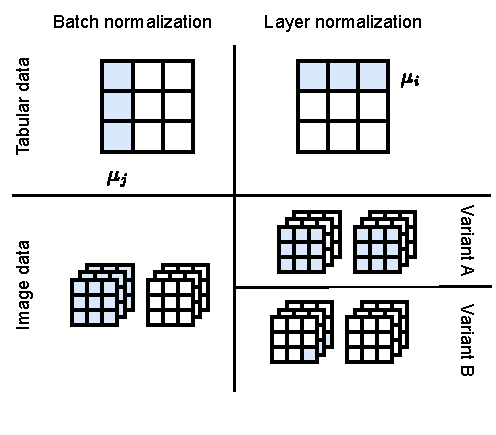
\includegraphics[width=0.6\textwidth]{images/layer_normalization}
    \caption{Comparison between BN and LN for tabular and image data. Blue regions show the sets over which we compute means and variances. For LN we have two variants, discussed better in the main text.}
    \label{fig:layer_normalization}
\end{SCfigure}

Consider Figure \ref{fig:layer_normalization}, where we show a comparison between BN and LN for tabular and image-like data. In particular, we show in blue all the samples used to compute a single mean and variance. For layer normalization, we can compute the statistics on $h,w,c$ simultaneously (variant A) or for each spatial location separately (variant B). The latter choice is common in transformer models, discussed in the next chapter. Other variants are also possible, e.g., \textbf{group normalization} restricts the operation to a subset of channels, with the case of a single channel known as \textbf{instance normalization}.\footnote{See \url{https://iclr-blog-track.github.io/2022/03/25/unnormalized-resnets/} for a nicer variant of Figure \ref{fig:layer_normalization}.}

In BN, the axes across which we compute the statistics in \eqref{eq:empirical_mean} and \eqref{eq:empirical_variance} are the same as the axes across which we apply the trainable parameters. In LN, the two are decoupled. For example, consider a PyTorch LN layer applied on mini-batches of dimension $(b, 3, 32, 32)$:

{\footnotesize
\noindent\mintinline{python}{ln = nn.LayerNorm(normalized_shape=[3, 32, 32])}
}

This corresponds to variant A in Figure \ref{fig:layer_normalization}. In this case, $\alpha$ and $\beta$ will have the same shape as the axes over which we are computing the normalization, i.e., $\alpha, \beta \sim (3,32,32)$, for a total of $2\times3\times32\times32=6144$ trainable parameters. The specific implementation of LN and BN must be checked for each framework and model.

We close by mentioning another common variant of layer normalization, called \textbf{root mean square} normalization (RMSNorm) \cite{zhang2019root}. It simplifies LN by removing the mean centering and shifting, which for a single input vector $\mathbf{x} \sim (c)$ can be written as:
%
\begin{equation}
\text{RMSNorm}(\mathbf{x}) = \frac{\mathbf{x}}{\sqrt{\frac{1}{c}\sum_i x_i^2}} \odot \mathbf{\alpha} 
\end{equation}
%
When $\mathbf{\beta} = 0$ and the data is already zero-centered, LN and RMSNorm are identical.

\section{Residual connections}
\label{sec:residual_connections}
\subsection{Residual connections and residual networks} \addclock

The combination of all techniques seen in the previous section is enough to increase significantly the number of layers in our models, but only up to a certain upper bound. Consider three generic sequence of layers $f_1$, $f_2$, and $f_3$, and two models where one is a subset of the other:
%
\begin{gather*}
g_1(x) = (f_3 \circ f_1)(x) \\ g_2(x)=(f_3\circ {\color{drawred}f_2}\circ f_1)(x)
\end{gather*}
%
Intuitively, by the universal approximation theorem it should always be possible for the intermediate part, $f_2$, to approximate the identity function $f_2(x) \approx x$, in which case $g_2(x) \approx g_1(x)$. Hence, there is always a setting of the parameters in which the second (deeper) model should perform at least as well as the first (shallower) one. However, this was not observed in practice, as shown in Figure \ref{fig:resnet}.

\begin{SCfigure}
    \centering
    \hspace{1em}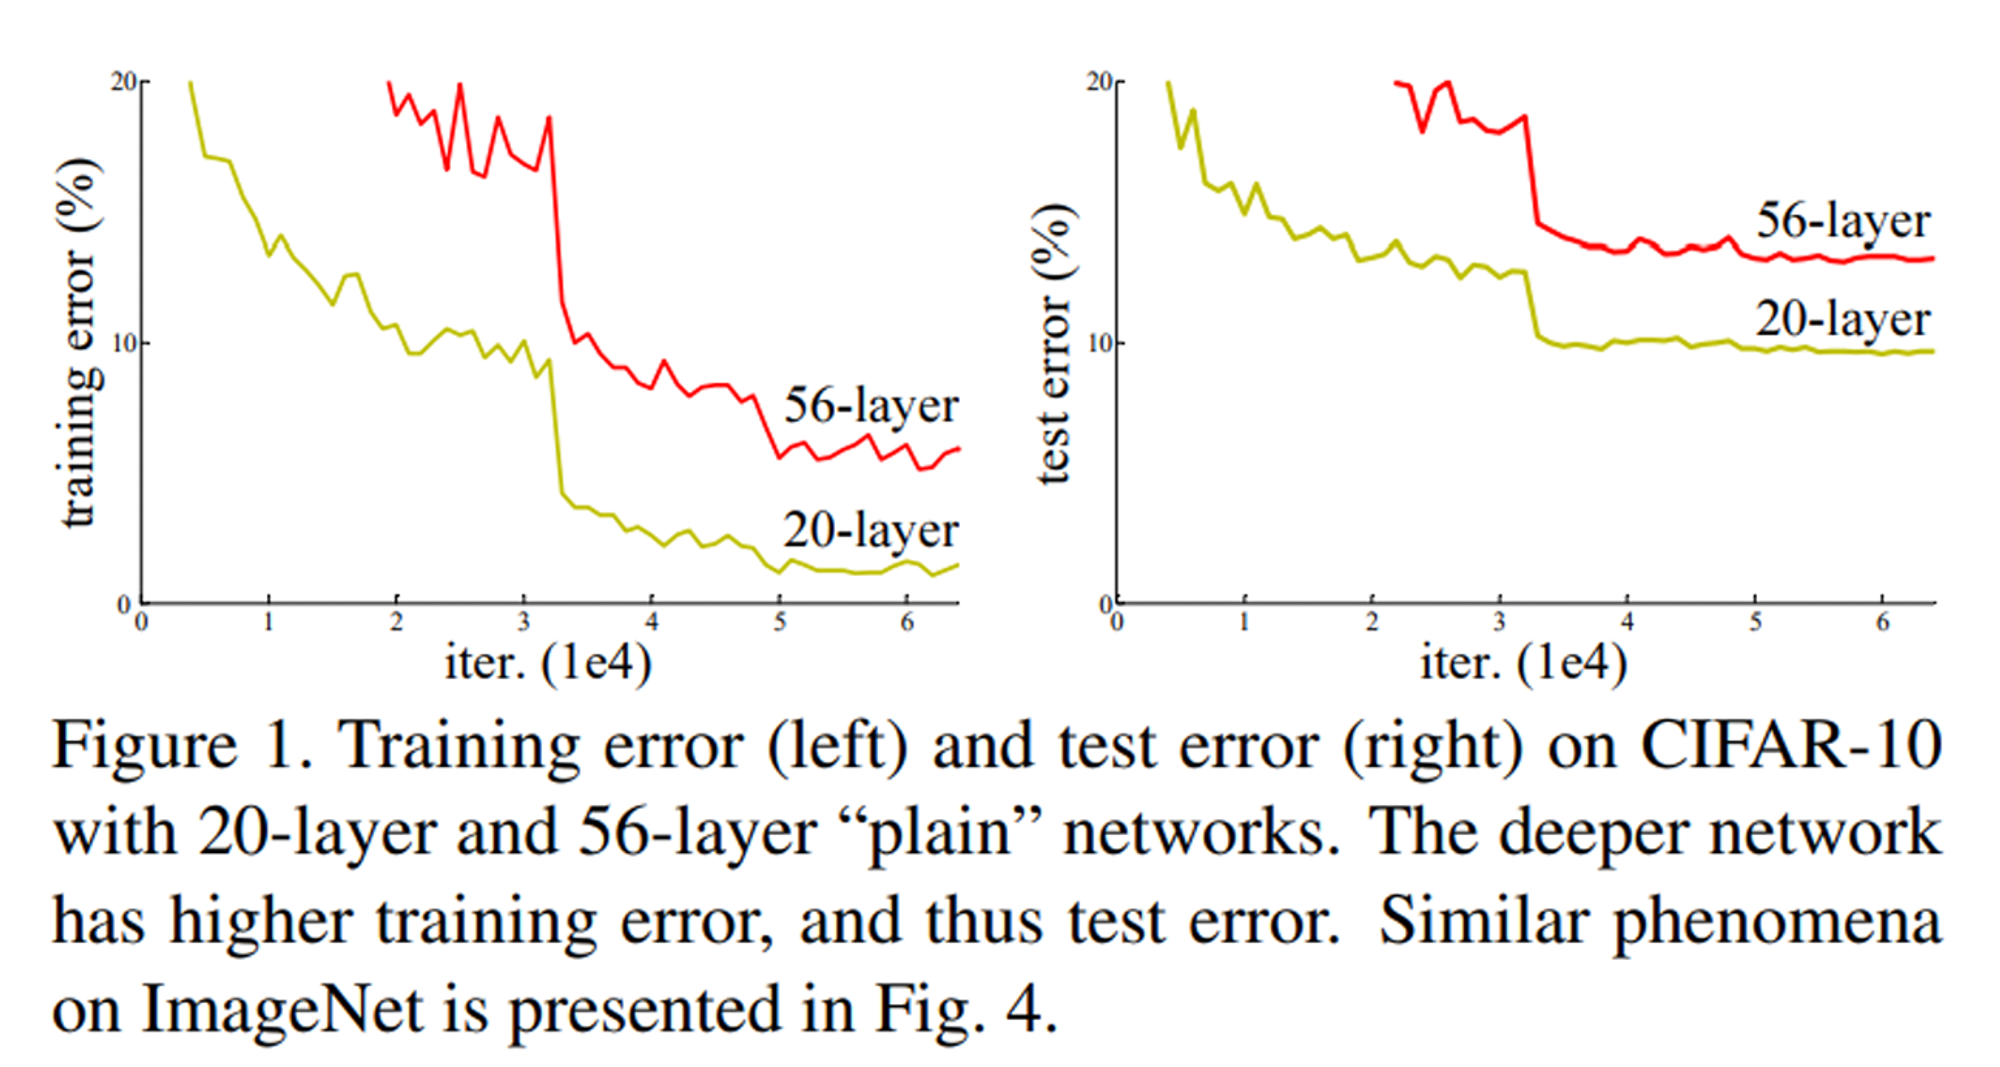
\includegraphics[width=0.6\textwidth]{images/resnet}
    \caption{Bigger models do not always improve monotonically in training error, despite representing larger classes of functions. Reproduced from \cite{he2016deep}.}
    \label{fig:resnet}
\end{SCfigure}

We can solve this by biasing the blocks in the network towards the identity function. This can be done easily by rewriting a block $f(x)$ with what is called a \textbf{residual (skip) connection} \cite{he2016deep}:
%
$$
r(x)=f(x){\color{drawred} \; + \;x}
$$
%
Hence, we use the block to model deviations from the identity, $f(x) = r(x) - x$, instead of modeling deviations from the zero function. This small trick alone helps in training models up to hundreds of layers. We call $f(x)$ the \textbf{residual path}, $r(x)$ a \textbf{residual block}, and a convolutional model composed of residual blocks a \textbf{residual network} (abbreviated to ResNet).

Residual connections work well with batch normalization on the residual path, which can be shown to further bias the model towards the identity at the beginning of training \cite{de2020batch}. However, residual connections can be added only if the input and output dimensionality of $f(x)$ are identical. Otherwise, some rescaling can be added to the residual connection. For example, if $x$ is an image and $f(x)$ modifies the number of channels, we can add a $1 \times 1$ convolution:
%
$$
r(x)=f(x)+\text{Conv2D}_{1\times 1}(x)
$$
%
The benefit of a residual block can be understood also in terms of its backward pass. Consider the VJP of the residual block:
%
$$
\text{vjp}_r(\mathbf{v})=\text{vjp}_f(\mathbf{v}) + \mathbf{v}^\top\mathbf{I} = \eqnmarkbox[drawred]{node}{\text{vjp}_f(\mathbf{v})} + \eqnmarkbox[drawgreen]{node2}{\mathbf{v}^\top}
$$
\annotate[yshift=-1em]{below,left}{node}{VJP of $f$}
\annotate[yshift=-3em]{below,left}{node2}{VJP of the skip connection}

\vspace{2em}
Hence, the forward pass lets the input $x$ pass through unmodified on the skip connection, while the backward pass adds the unmodified back-propagated gradient $\mathbf{v}$ to the original VJP, which can help mitigating gradient instabilities.

\subsection*{On the design of the residual block}

How to design the block $f(x)$? Consider the batch-normalized block introduced earlier:
%
$$
h = \underbrace{(\text{ReLU}\circ \text{BN} \circ \text{Conv2D})}_{=f(x)}(x) + x
$$
%
Because the output of ReLU is always positive, we have that $h \ge x$ (element-wise). Hence, a stack of residual blocks of this form can only increase the values of the input tensor, or set it to zero. For this reason, the original design proposed in \cite{he2016deep} considered a stack of blocks of this form by removing the last activation function. As an example, for two blocks we obtain the following design:
%
$$
h = (\text{BN} \circ \text{Conv2D} \circ\text{ReLU}\circ \text{BN} \circ \text{Conv2D})(x) + x
$$
%
A series of blocks of this form can be preceded by a small component with non-residual connections to reduce the image dimensionality, sometimes called the \textbf{stem}. The specific choice of hyper-parameters for this block has varied significantly over the years.

\begin{SCfigure}
    \centering
    \hspace{1em}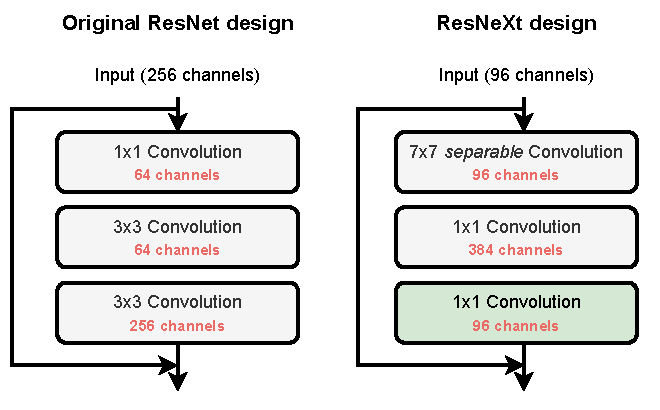
\includegraphics[width=0.6\textwidth]{images/resnet_design}
    \caption{The original ResNet block \cite{he2016deep}, and the more recent ResNeXt \cite{liu2022convnet} block. As can be seen, the design has shifted from an early channel reduction to a later compression (\textbf{bottleneck}). Additional details (not shown) are the switch from BN to LN and the use of GELU activation functions. Adapted from \cite{liu2022convnet}.}
    \label{fig:resnext}
\end{SCfigure}

The original ResNet block proposed a compression in the number of channels for the first operation, followed by a standard $3 \times 3$ convolution and a final upscaling in the number of channels. Recently, instead, \textbf{bottleneck} layers like the  v block \cite{liu2022convnet} (on the right in Figure \ref{fig:resnext}) have become popular. To increase the receptive field of the convolution, the initial layer is replaced by a depthwise convolution. To exploit the reduced number of parameters, the number of channels is \textit{increased} by a given factor (e.g., $3\times$, $4\times$), before being reduced by the last $1\times1$ convolution.

\subsection{Additional perspectives on residual connections} \addteacup

We close the chapter by discussing two interesting perspectives on the use of residual connections, which have both been explored in-depth in current research. First, consider a network composed of two residual blocks:
%
\begin{gather}
h_1 = {\color{drawred}f_1}(x)+x\\h_2={\color{drawgreen}f_2}(h_1)+h_1
\end{gather}
%
If we unroll the computation:
%
$$
h_2 = {\color{drawgreen}f_2}({\color{drawred}f_1}(x) + x) + {\color{drawred}f_1}(x) + x
$$
%
This corresponds to the sum of several \textit{paths} in the network, where the input is either left unmodified, it goes through only a single transformation ($f_1$ or $f_2$), or through their combination.

\begin{SCfigure}
    \centering
    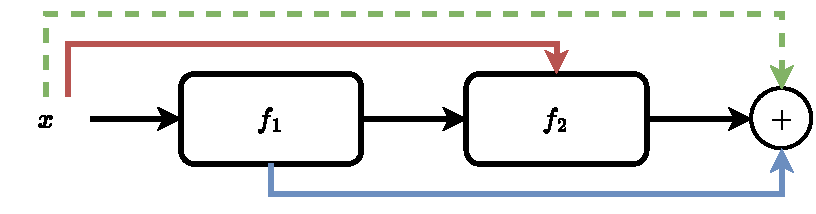
\includegraphics[width=0.6\textwidth]{images/residual_paths}
    \caption{Residual paths: the black, red, and blue paths are implemented explicitly; the green path is only implicit.}
    \label{fig:residual_paths}
\end{SCfigure}

It should be clear that the number of such paths grows exponentially with the number of residual blocks. Hence, deep residual models can be seen as a combination (an ensemble) of a very large number of smaller models, implemented through weight-sharing. This view can be tested to show, for example, that ResNets tend to be robust to small deletions or modifications of their elements \cite{veit2016residual}. This is shown visually in Figure \ref{fig:residual_paths}.

Second, consider the following differential equation, expressed in terms of a continuous parameter $t$ representing time:
%
$$
\partial_tx_t=f(x,t)
$$
%
We are using a neural network with arguments $x$ and $t$ (a scalar) to parameterize the time derivative of some function. This is called an \textbf{ordinary differential equation} (ODE). A common problem with ODEs is integrating from a known starting value $x_0$ up to some specified time instant $T$:
%
$$
x_T=x_0+\int_{t=0}^Tf(x,t)dt
$$
%
Euler's method\footnote{\url{https://en.wikipedia.org/wiki/Euler_method}} for computing $x_T$ works by selecting a small step size $h$ and computing iteratively a first-order discretization:
%
$$
x_t=x_{t-1}+hf(x_{t-1}, t)
$$
%
Merging $h$ into $f$, this corresponds to a restricted form of residual model, where all residual blocks share the same weights, each layer corresponds to a discretized time-instant, and $x_T$ is the output of the network. Under this point of view, we can directly work with the original continuous-time equation, and compute the output by integrating it with modern ODE solvers. This is called a \textbf{neural ODE} \cite{chen2018neural}. Continuous-time variants of back-propagation can be derived that take the form of another ODE problem. We will see in the next volume an interesting connection between neural ODEs and a class of generative models known as \textbf{normalizing flows} \cite{papamakarios2021normalizing}.

\section*{From theory to practice}

\begin{wrapfigure}{r}{3.0cm}
\vspace{-3em}
\includegraphics[width=3.0cm]{images/shutterstock_2075221579.jpg}
\vspace{-2em}
\end{wrapfigure}

All the layers we discussed in this chapter (batch normalization, dropout, ...) are already implemented in PyTorch, Equinox, and practically every other framework. For what concerns the rest of the techniques we described, it depends on the framework: for example, weight decay in implemented natively in all PyTorch's optimizers, data augmentation can be found as transformations inside \texttt{torchvision} (and other corresponding libraries), while early stopping must be implemented manually.\footnote{In PyTorch, a common alternative is to use an external library such as PyTorch Lightning to handle the training process. Modifications to the training procedure, such as early stopping, are pre-implemented in the form of \textit{callback} functions.}

\begin{enumerate}
\item Before proceeding to the next chapter, I suggest you try implementing either dropout or batch normalization as a layer using only standard linear algebra routines, comparing the results with the built-in layers.
\item In Chapter \ref{chap:cnns} you should have implemented a simple convolutional model for image classification. Try progressively increasing its size, adding normalization, dropout, or residual connections as needed.
\item Take a standard architecture, such as a ResNet \cite{he2016deep}, or a  ResNeXt \cite{liu2022convnet}. Try implementing the entire model by following the suggestions from the original papers. Training on ImageNet-like datasets can be challenging on consumer's GPU -- if you do not have access to good hardware or cloud GPU hours, you can keep focusing on simpler datasets, such as CIFAR-10.
\item At this point, you may have realized that training from scratch very large models (e.g., ResNet-50) on smaller datasets is practically impossible. One solution is to initialize the weights of the model from an online repository using, e.g., the weights of a model trained on ImageNet, and \textbf{fine-tuning} the model by modifying the last layer, corresponding to the classification head. By this point of the book, this should come as relatively easy -- I suggest using one of the many pre-trained models available on torchvision or on the Hugging Face Hub.\footnote{For an example tutorial: \url{https://pytorch.org/tutorials/beginner/transfer_learning_tutorial.html}.} We will cover fine-tuning more in-depth in the next volume.

\end{enumerate}